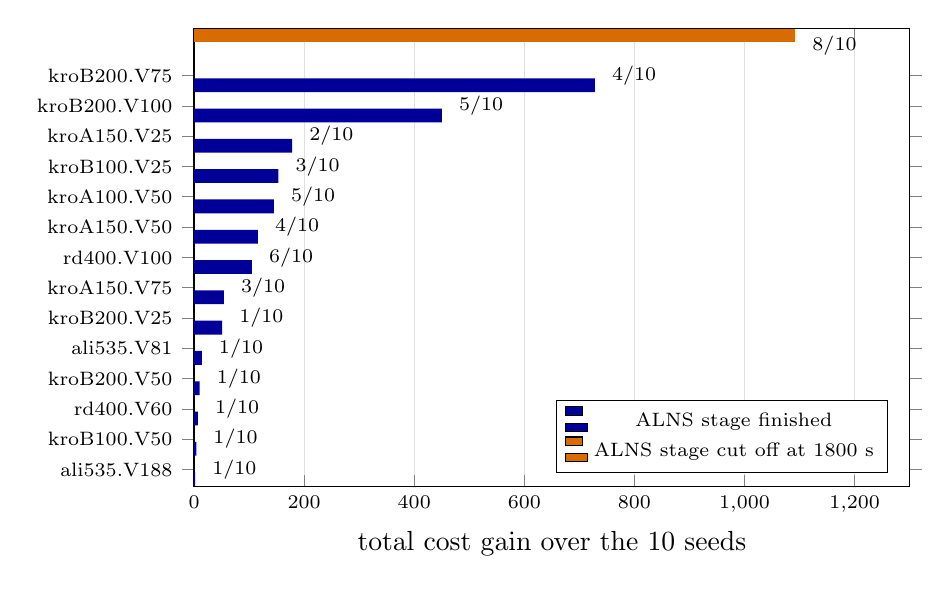
\begin{tikzpicture}
\begin{axis}[xbar,width=0.88\textwidth,height=7.4cm,bar width=5pt,
  symbolic y coords={ali535.V188,kroB100.V50,rd400.V60,kroB200.V50,ali535.V81,kroB200.V25,kroA150.V75,rd400.V100,kroA150.V50,kroA100.V50,kroB100.V25,kroA150.V25,kroB200.V100,kroB200.V75,rd400.V140},ytick=data,y tick label style={font=\scriptsize},
  x tick label style={font=\scriptsize},xlabel={total cost gain over the 10 seeds},xmin=0,xmax=1300,
  enlarge y limits=0.04,legend pos=south east,legend style={font=\scriptsize},
  xmajorgrids,major grid style={gray!25}]
\addplot[fill=blue!60!black,draw=none] coordinates {(2,ali535.V188) (4,kroB100.V50) (7,rd400.V60) (10,kroB200.V50) (14,ali535.V81) (51,kroB200.V25) (54,kroA150.V75) (105,rd400.V100) (116,kroA150.V50) (145,kroA100.V50) (153,kroB100.V25) (178,kroA150.V25) (450,kroB200.V100) (728,kroB200.V75)};
\addplot[fill=orange!85!black,draw=none] coordinates {(1092,rd400.V140)};
\legend{ALNS stage finished,ALNS stage cut off at 1800 s}
\node[font=\scriptsize,anchor=west] at (axis cs:2,ali535.V188) {~1/10};
\node[font=\scriptsize,anchor=west] at (axis cs:4,kroB100.V50) {~1/10};
\node[font=\scriptsize,anchor=west] at (axis cs:7,rd400.V60) {~1/10};
\node[font=\scriptsize,anchor=west] at (axis cs:10,kroB200.V50) {~1/10};
\node[font=\scriptsize,anchor=west] at (axis cs:14,ali535.V81) {~1/10};
\node[font=\scriptsize,anchor=west] at (axis cs:51,kroB200.V25) {~1/10};
\node[font=\scriptsize,anchor=west] at (axis cs:54,kroA150.V75) {~3/10};
\node[font=\scriptsize,anchor=west] at (axis cs:105,rd400.V100) {~6/10};
\node[font=\scriptsize,anchor=west] at (axis cs:116,kroA150.V50) {~4/10};
\node[font=\scriptsize,anchor=west] at (axis cs:145,kroA100.V50) {~5/10};
\node[font=\scriptsize,anchor=west] at (axis cs:153,kroB100.V25) {~3/10};
\node[font=\scriptsize,anchor=west] at (axis cs:178,kroA150.V25) {~2/10};
\node[font=\scriptsize,anchor=west] at (axis cs:450,kroB200.V100) {~5/10};
\node[font=\scriptsize,anchor=west] at (axis cs:728,kroB200.V75) {~4/10};
\node[font=\scriptsize,anchor=west] at (axis cs:1092,rd400.V140) {~8/10};
\end{axis}
\end{tikzpicture}
